%!TEX root = ../thesis.tex
% Pipeline of the DemoDraw system: technical details

\begin{figure}[t]
  \centering
  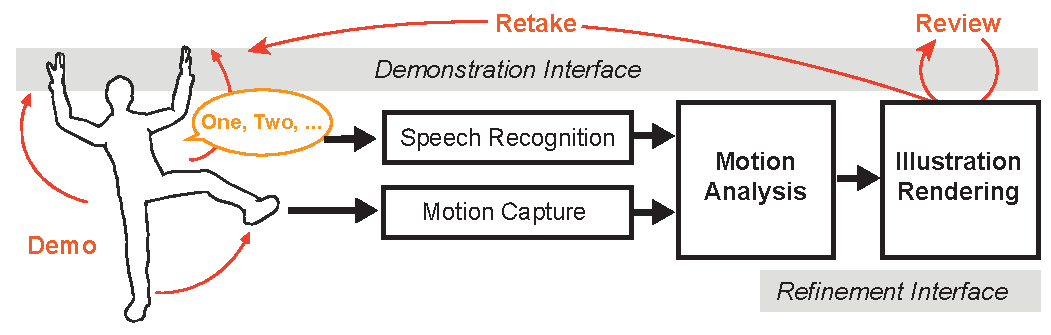
\includegraphics[width=1.0\columnwidth]{\demodraw/fig/pipeline/pipeline}
  \caption{\systemname{} System Components and Pipeline}
  % \dan{now that I understand the components better, we should emphasize motion capture component less since didn't make much contribution there.  I tweaked the figure to do this, and also highlighted the ``interaction pipeline'' (demo, review, retake) a bit better too.   }
  \label{fig:pipeline}
\end{figure}

\section{Automatic Generation Pipeline}

% \dan{I think we should downplay ``pipeline'' and emphasize ``system components'' ... pipeline sound very linear and non-iterative.}

%To support the described user scenario, we introduce our pipeline and system components shown in .
\systemname{} has four main components (Figure~\ref{fig:pipeline}):
%
a \emph{motion capture} engine to record joint data from the author's demonstration and map it data to a 3D avatar;
%
a \emph{speech recognition} engine to process speech input for commands and motion labels;
%
a \emph{motion analysis} algorithm that segments recorded motion and identifies salient joint movements for each illustration panel;
%
and an \emph{illustration rendering} engine to visualize the avatar and motion segments with different effects.
% , and a module to handle user interaction.
%
% Our novel techniques enables motion segmentation by combining speech and motion inputs. Our interaction model allows users to modify the rendered illustrations interactively by demonstrations.
The combination of these components enables an interactive and iterative system pipeline to translate demonstrations into motion diagrams.
A notable technical contribution is our motion segmentation algorithm leveraging parallel speech label and joint motion input streams.
% \dan{I tweaked the two points above, old text is commented out in the tex}

% \dan{say something like our technical contribution is in motion segmentation (and maybe illustration rendering) }
%
\systemname{} is implemented using C\# in Unity 5\footnote{\url{https://unity3d.com}}.
It runs interactively on a Macbook Pro with Windows Bootcamp (2.5 GHz Intel Core i7 processor and 16 GB memory).
%
Below we describe the design and implementation of each component.

% ---------------------------------------------------------------

\subsection{Motion Capture}
% \dan{Call it ``Motion Capture'' component, with three sub components: Kinect, Avateering, and NPR}
% \bjoern{I moved NPR from capture to illustration rendering since it's a rendering technique.}
% \dan{good idea}

In support of our design goal to enable low-effort iteration within tasks, the motion capture component provides real-time feedback during demonstrations so authors can monitor their performance accordingly.
%\fixme{The raw joint data and RGB video stream are saved as csv and mp4 files for retrieval.}
%\dan{I put this here, but not sure we really need to state it at all. We don't really use the RBD video for anything either.}
% A central goal of our system is to enable average users to create illustration by physical demonstrations. As users might not necessarily have expertise to design illustration outcomes prior to a performance, it is important to provide real-time feedback for authors to observe the continuous motion captured effect and perform accordingly.
%
%\subsubTitleBold{Real-time Joint Data}
We capture position and joint angles of a simplified 25-joint skeleton using a Kinect2 sensor and the Kinect SDK 2.0\footnote{\url{https://dev.windows.com/en-us/kinect}}.
%Skeletal data of human body's 25 joints is captured in 3D, including head, shoulders, hands, and foot.
% At any given frame of motion capturing, our system gathers information about position, depth, and orientation values in meters for each of the 25 joints.
%Therefore, \systemname{} presents a 3D human model mirroring an author's movements in real-time while she stands in front of a Kinect sensor in a static, indoor scene (Figure~\ref{fig:pipeline}a).
%\dan{I commented a lot out here it didn't seem to add much beyond ``we capture using a Kinect'' (and just saying something like that is ok). }
%
%\subsubTitleBold{Motion Re-targeting}
The real-time joint data is applied to a generic 3D human model (an ``avatar'') using forward kinematics enabled by a modified Unity asset\footnote{\url{https://www.assetstore.unity3d.com/en/\#!/content/18708}}.
% \dan{I commented out a vague description of forward kinematics, I don't think we need it.}
% \bjoern{So the use of ``retargeting'' kinda raises a whole bunch of issues since motion retargeting is a big topic in animation. If bone lengths don't match between the actor's skeleton and the virtual model, contacts like clap or hand-on-head won't work. At a minimum state that we do not yet perform any smart retargeting to deal with changing segment lengths. I think the canonical reference is Gleicher~\cite{gleicher1998retargetting}.}
% \dan{yes, let's avoid saying ``retargeting''}

% When the motion data gets updated from the Kinect sensor, \systemname{} applies the joint information to a structured 3D human model (i.e., an ``avatar'') using forward kinematics in real-time. Given the human skeleton hierarchy from the body root (i.e., base spine) to the end of body parts (such as hand tips and feet), we compute the bone rotation angle to locate each joint to the target location in space. In this way, user can observe the avatar that follows her motion, which can also be viewed from any angle in a 3D space. This can be useful when user performs movements perpendicular to the Kinect camera \peggy{need a better way to frame this}.


% Based on our survey on existing practices of illustration design principles, it is important to make a character's appearance concise and clean. Often, outlining a human figure or showing in silhouette effectively preserves only essential information. Therefore, we apply Non-Photorealistic Rendering (NPR) techniques \cite{gooch1998non} to the 3D avatar in our engine that can be rendered and modified in real-time, including outline, silhouette, and flat-shaded colour (see Figure~\ref{fig:DemoDrawUI}-1d for examples).
% quaternion

% \subsubTitleBold{Implementation}
% This engine is implemented using Unity 5\footnote{\url{https://unity3d.com}} and the Kinect SDK 2.0 package\footnote{\url{https://dev.windows.com/en-us/kinect}} in C\#. Raw joint data and video stream from color frames are saved as csv and mp4 files for retrieval. Motion retargeting is achieved by a modification of a Unity asset\footnote{\url{https://www.assetstore.unity3d.com/en/\#!/content/18708}}. NPR shaders are applied to the 3D model for different rendering results.

% ---------------------------------------------------------------

\subsection{Speech Recognition}
Speech is used when recording a demonstration to label motions (e.g., ``one, two, ...'') and for recording and navigation commands (e.g. ``start, stop'' or ``three, back'' to skip to a motion segment) -- see Figure~\ref{fig:DemoDrawUI} for the speech commands that \systemname{} supports.
%
We recognize both types of speech using the Microsoft speech recognition library\footnote{\url{https://msdn.microsoft.com/en-us/library/hh361572}} to process audio captured by the Kinect microphone array.
During recording, the time stamp, delay, and confidence of motion labels are logged for use in the the motion analysis algorithm.
% \dan{how do you calculate delay? I thought this was a fixed constant determined by manual inspection.}
% \peggy{The api provides, but I didn't get to use it...}

%In addition, \fixme{a set of X voice commands} are recognized for non-sequential navigation .

%  addition to capturing and rendering user's continuous movements, \systemname{} considers instructor's existing practices of specifying motions using speech during a physical demonstration.
% By listening to the Kinect sensor's microphone array, \systemname{} integrates a speech recognition engine\footnote{\url{https://msdn.microsoft.com/en-us/library/hh361572}} to recognize user's speech input in real-time. Information of a detected spoken word, including the timestamp, delay, and confidence, is captured to be used for motion analysis and to support \systemname{}'s multi-modal interaction.
%
% Can implement: go more than one word and combine (e.g., turn to the right)

% ---------------------------------------------------------------

\subsection {Motion Analysis}
% \dan{Would be good to get a component name to include joint salience identification too.  ``Motion Segmentation and Joint Salience Identification'' component is too long, how about something more simple and general like ``Motion Analysis'' with subcomponents motion segmentation and joint salience.}

Our motion analysis algorithm translates a multi-part demonstration recording into a sequence of labeled time segments, each with one or more salient joint motions and a keyframe of joint positions to use as a representative body pose (see Figure~\ref{fig:segmentation} for an illustration of the approach).
Formally, the algorithm associates each speech label with a motion start and end time [$T_s$, $T_e$], set of salient joints ${J_0, ..., J_n}$, and keyframe time $T_k$.
Each segment is sent to the Illustration Rendering engine to create each motion illustration in a multi-part sequence.

Human motion segmentation and activity understanding has been well studied in computer vision and graphics \cite{Aggarwal:2011:HAA:1922649.1922653}. We adopted a time-space approach to identify salient motion sequences in 3D space.
%
In our scenario, each movement may not be necessarily seen or labeled with a semantic meaning (such as ``running'' or ``walking'' in previous research). Therefore, our approach combines speech labeling from a user, similar to the scene segmentation method used by \cite{chi2013democut}.
%
We make three assumptions about the synchronized data streams of speech labels and joint movements:
authors make short pauses between motions to be grouped;
the speech label utterances overlap or closely occur with at least one joint motion;
step-by-step movements are clearly segmented without an overlap.
%
These assumptions are practical as authors often pause for a moment to prepare for demonstrating the next movement in a step-by-step sequence.
% , or reposition their body without those movements being assigned to any label.

% where $T_s \leq T_w \leq T_e$,


% For a motion label detected by the speech recognition engine at time \(T_w\) (e.g., step ``One'' or a gesture ``Swipe''), \systemname{} automatically identifies an appropriate motion segment for visualization as follows: It analyzes the motion data in order to identify the start and end time of this segment [\(T_s\), \(T_e\)] where \(T_s \leq T_w \leq T_e\), a set of salient joints \({J_0, ..., J_n}\), and a representative pose at \(T_k\) associated with this speech label. Figure~\ref{fig:segmentation} shows one example of a right-hand movement segmented by the following approach: \bjoern{What instant in time does \(T_w\) represent? The beginning of a word? The end? Some time after the end of the word once recognition has completed? Seems fairly important - otherwise I have no idea if \(T_s \leq T_w \leq T_e\) is a reasonable assumption.}


% EUCLIDEAN DISTANCE
\subsubTitleBold{Motion Segmentation}
Let $T_w$ be the delay-corrected time when a speech label like \iquote{one} was detected.
The first operation is to determine [$T_s$, $T_e$] for each speech label such that $T_s - \epsilon \leq T_w \leq T_e + \epsilon$, where $\epsilon$ is set to be 1 second to allow short pauses between speech and movement.
%
The operation begins by identifying periods of significant joint movement for 8 joints: the 5 end-effectors (head, hands, feet), 2 knees, and the body root.
%
To filter jittery movements, joints are considered moving if smoothed inter-frame differences in absolute Euclidean distance are greater than a threshold.
%
Specifically, for each joint $J_i$ at time $t$, the average difference in position between two adjacent frames $\Delta P = |P_t-P_{t-1}|$ is computed over the subsequent half second (15 frames).
%
If this moving average is greater than 0.05$meter/s$, then joint $J_i$ is labeled as ``moving'' at time $t$, marked as $m_i^t$.
This is repeated on all frames and all joints to find all periods of significant joint movement (pink rectangles in Figure~\ref{fig:segmentation}).
% \dan{any extra hacks to join or filter out very small periods of movement like just a few frames? If so, explain here.}

Next, after combining all the consecutive $m_i^{T_s}, m_i^{T_s+1}, ..., m_i^{T_e}$ between time [$T_s$, $T_e$] for joint $J_i$, we begin labeling each joint moving period $M_i$:
%
Given a list of speech labels, for each speech label at time $T_w$, label any unmapped period $M_i$ of joint \(J_i\) where $T_s - \epsilon \leq T_w \leq T_e + \epsilon$ (i.e., the speech utterance is detected during or closely occur with a joint movement, illustrated as dashed lines crossing pink rectangles in Figure~\ref{fig:segmentation}).
%
% Salient joint marking covered in the next paragraph ...
%Mark \(J_i\) as salient.
%
% If a movement overlaps with two labels (i.e., a continuous movement without a pause in between beyond our general assumption),
%
% \dan{do you have any rules to prevent a period of joint movement to be mapped to multiple speech labels?}
%
% Any unmapped periods ending less than $\epsilon$ before a motion label time, where $\epsilon = $ 1s defined earlier, or beginning less than $\epsilon$ after a motion label time, are also mapped to that label.
% \dan{See if what I wrote above makes sense, I was trying to interpret ``or 2) if an earlier segment that ends within a pause threshold is not mapped. A second pass of analysis after recording will examine if a segment shown after the label should be mapped to this label.'' }
%
% \fixme{After all the moving sequences of a joint is identified, \systemname{} concatenates these elements and finds the earliest frames at \(T_s\) and latest frame at \(T_e\) as the start and end times of this motion segment. Mark this as a salient joint \(J_i\).} \bjoern{revisit - i find this unclear, but I'm also tired.}\dan{I can't figure it out either, but I think it needs to be explained here}
%
Once all periods of joint movement are mapped to labels for all major joints, the motion segment start time and end time [$T_s,T_e$] are set to the minimum start time and maximum end time across all mapped joint movement periods.
% \dan{the sentence above is my guess at what this means (same as what Bjoern guessed)
% ``Our algorithm repeats this segmentation for all the major joints. If there are multiple salient joints, combine and adjust [\(T'_s\), \(T'_e\)] for this motion segment.'' \bjoern{How do you do the adjustment? do different joints have individual start and end times, or do you take the min of all start times and the max of all end times?}}

\subsubTitleBold{Joint Salience Identification}
The salient joints for a segment is the set of all joints \(J_i\) that were mapped based on significant motion segments.
% \dan{any other rules or hacks to do this?}

% \systemname{} analyzes a motion recording for significant motion changes using spatial thresholding of key joints. To concisely visualize body motion, we selected a subset from the 25 joints by their relative distance of a human body. For example, shoulder center can be represented by the head movement, and therefore trace only the latter joint. \bjoern{This is vague - which joints did you select? Why is this ``concise''? I don't understand the sentence about shoulders and heads at all. Maybe show a figure and highlight which joints you check.}
%
% For each joint, we calculate the Euclidean distance of joint locations in adjacent frames: $\Delta P = |P_t-P_{t-1}|$. If the average distance of a consecutive sequence within a moving window (set as 2 seconds) is over a difference threshold, it labels this as a moving joint sequence. \bjoern{what do you mean by average distance? do you just add up all frame differences for 2 seconds and divide by \# of frames? What is the difference threshold you empirically determined? What are the times $[T_{start},T_{end}]$ you find? }

% MATCH WITH SPEECH + FIND IN/OUT POINTS
% Next, our algorithm maps a moving joint sequence to this speech label if: 1) the sequence in time overlaps with the label's time \(T_w\), i.e., the movement is continuing, or 2) if an earlier segment that ends within a pause threshold is not mapped. A second pass of analysis after recording will examine if a segment shown after the label should be mapped to this label.
% %
% After it identifies all the moving sequences of a joint, \systemname{} concatenates these elements and finds the earliest frames at \(T_s\) and latest frame at \(T_e\) as the start and end times of this motion segment. Mark this as a salient joint \(J_i\). \bjoern{revisit - i find this unclear, but I'm also tired.}

% MULTIPLE JOINTS
% \subsubTitleBold{Joint Salience Identification}
% Our algorithm repeats this segmentation for all the major joints. If there are multiple salient joints, combine and adjust [\(T'_s\), \(T'_e\)] for this motion segment. \bjoern{How do you do the adjustment? do different joints have individual start and end times, or do you take the min of all start times and the max of all end times?}

% KEY FRAME
\subsubTitleBold{Key Pose Selection}
We use a time near the end of each segment as the representative pose keyframe, specifically $T_k = T_e - 1$ second.
We experimented with other options including the middle of the segment, but found designers most often chose a pose near the end as the key frame.
% \dan{should mention keyframe position in formative study section}
% \peggy{confirmed, and in figure 2}
% Therefore, we selects a frame \bjoern{x frames} from the out point \peggy{no intelligence here... how do we better describe?}.

%\subsubTitleBold{Segment Retake}
% \dan{I added the last part of that sentence, it works like that, right?}
% \peggy{If pauses are long enough}
When retaking a partial demonstration with one or more speech labels, the full motion analysis algorithm is run on the new recording, and new motion segments are inserted into the sequence of labeled time segments. %(see Figure~\ref{fig:segmentation}B).

% ---------------------------------------------------------------

\subsection{Illustration Rendering}

The Illustration Rendering engine generates a motion illustration for each segment of joint motion (bounded by [$T_s$, $T_e$]). There are two related rendering tasks: the body pose and the motion depiction style.

\subsubTitleBold{Body Pose}
Following the principle of clarity through simplicity, Non-Photorealistic Rendering  \cite{gooch1998non} algorithms are used to render the 3D human model as an outline, silhouette, or flat-shaded colour (see Figure~\ref{fig:DemoDrawUI}c left for examples).
The body pose is determined by all joint positions at keyframe time $T_k$.
% \dan{any more details? Unity asset used? tuning parameters? Is it fast?}

\subsubTitleBold{Line and Arrow Depiction Style}
Based on Cutting's criteria~\cite{cutting_representing_2002} and our survey of motion illustrations, we use lines with arrowheads as the default depiction style for visualizing joint movements.
This style is rendered as follows:
%
For each salient joint \(J_i\) in \({J_0, ..., J_n}\) of a motion segment, the absolute joint positions in world space over the period [\(T_s\), \(T_e\)] are used to construct a 3D poly-line.
The default is to render a smooth poly-line by interpolating positions using Catmull-Rom.
% \dan{can smoothing still be turned off?}
% \peggy{current not}
Two 3D cones are positioned collinear with the last two polyline positions to form arrowheads for both the beginning and the end of a line.
%
Although the poly-line is constructed in 3D, it is rendered with shading to appear 2D.
% \dan{and rendered to be always ``in front'' of the body.}
% \peggy{currently does not consider camera viewpoint, so no}

% \dan{relative positions instead}
For some motions, visualizing absolute joint positions might not be suitable.
For example, for a two-foot jump with a two-hand waving motion (see Figure~\ref{fig:DemoDrawUI}c bottom), our algorithm will mark all major joints as salient and generate multiple arrows showing the jump movement, but failing to convey the hand waving.
%
Authors can choose to visualize joint motions \textit{relative} to the spine instead.
The same motion analysis algorithm described above can then be re-run using relative motion.
For the two-foot jump example, this would render a more concise illustration with a single up arrow (for the overall jump direction) and two curve arrows (for the hand movements).
%The joint data will be re-computed based on the offset distance to the spine position. The result illustration, in this case, can be more concise by showing only the spine motion.

Authors can review the results using both the \phaseI{} and \phaseII{}. With the latter, line weight, arrowhead sizes, and color can also be adjusted and re-rendered in real-time using a graphical interface (see Figure~\ref{fig:DemoDrawUI}c left). Arrows can also be re-positioned by direct manipulation dragging.

\subsubTitleBold{Stroboscopic Depiction Style}
Cutting~\cite{cutting_representing_2002} noted stroboscopic effects are also effective, and we found examples of illustrations with a sequence of overlaid semi-transparent body poses in our survey.
%
Therefore, authors can select a stroboscopic depiction style in the \phaseII{}.
The style is rendered by compositing multiple semi-transparent renderings of intermediate body poses between $T_s$ to $T_e$ behind a rendering of the representative pose at keyframe time $T_k$.
Authors can adjust the number of intermediate poses (the default is 3 poses) and the horizontal offset between each intermediate pose rendering can be adjusted to stack them up (zero offset by default) or spread them out.

% Authors can then selectively combine these frames by specifying visual parameters, including numbers of frames to show, distance between frames, and whether to apply motion arrows. Our system will automatically adjust the distance and transparency values of selected frames and compose into a diagram.

\subsection{Results}
The \systemname{} pipeline is capable of generating expressive and clear motion illustrations. In Figure~\ref{fig:demodraw_teaser}c, motion arrows show the upper body motion (top left), hand waving back and forth (top middle), and hand circular motion (bottom right). Whole body motions can also be visualized (bottom left), and can be especially helpful when motions are best viewed from a different angle, such as the side view (top right).
%
In Figure~\ref{fig:demodraw_teaser}d, stroboscopic effect depicts the transition from the start pose to the end pose, which can be rendered as a sequence (top left) or in one combined pose (bottom left). A combination of this effect with motion arrows enhances an illustration efficiently in an integrated figure (top and bottom right).

% \dan{Talk about how expressive this pipeline is referring to diagrams shown in figure 1, the appendix, etc.}

\dan{Disclose what happens if assumptions don't hold or other problems with the pipeline. (this paragraph may migrate elsewhere).}

% ---------------------------------------------------------------

\begin{figure}[t]
  \centering
  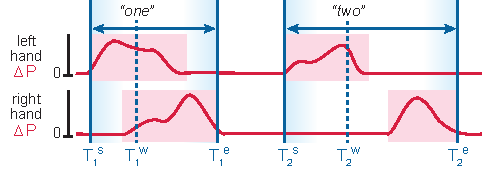
\includegraphics[width=1.0\columnwidth]{\demodraw/fig/motion_analysis/analysis2}
  \caption{Illustration of motion analysis algorithm (two joints shown due to space): significant periods of joint motion (pink) are mapped to speech labels to define motion segments (blue). Note the right hand period is mapped to \iquote{two} because it begins shortly after the left hand period.}
   \label{fig:segmentation}
\end{figure}

% \begin{figure}[t]
%   \centering
%   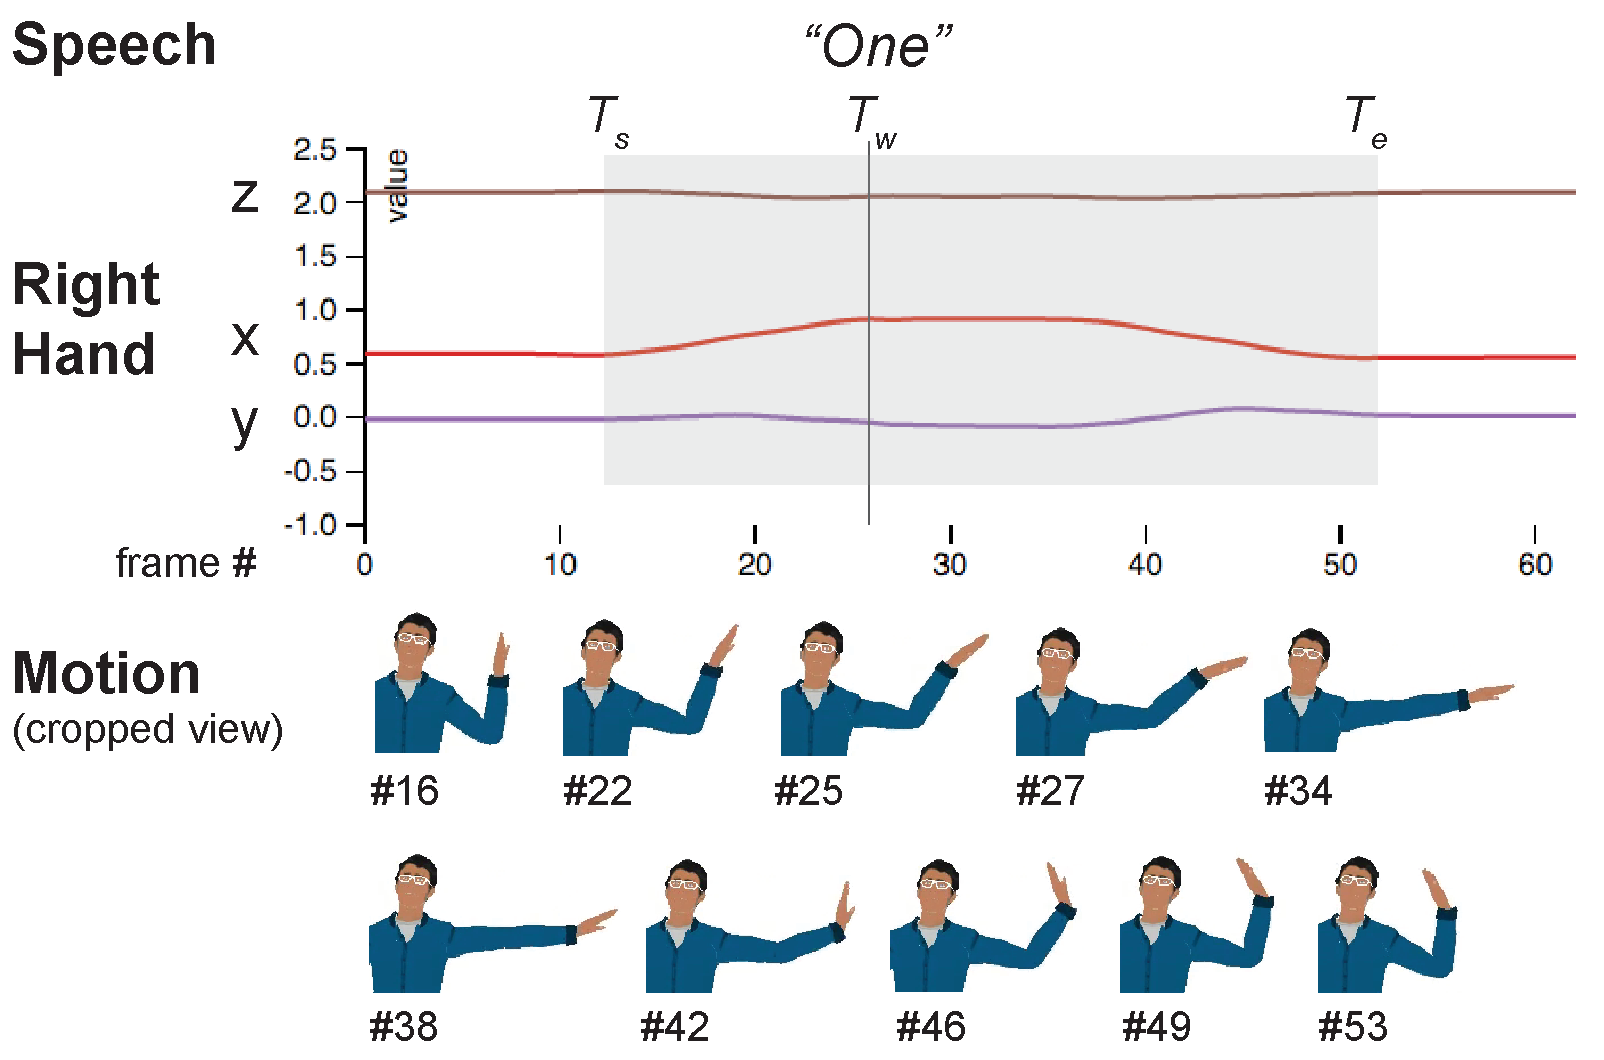
\includegraphics[width=1.0\columnwidth]{fig/motion_analysis/analysis}
%   \caption{Illustration of motion analysis algorithm (only one joint shown due to space): the significant joint motion period (gray) is mapped to the speech label \iquote{one}.}
%   \dan{I don't think this diagram is conveying as much information about the algorithm as it could. Showing more than 1 joint and more than 1 label would be better. The avatar pictures aren't really necessary, people will get the x,y,z graphs since we're talking about abstract position data anyway. See diagram sketch above.}
%   \label{fig:segmentation}
% \end{figure}



